\begin{figure}[h]
	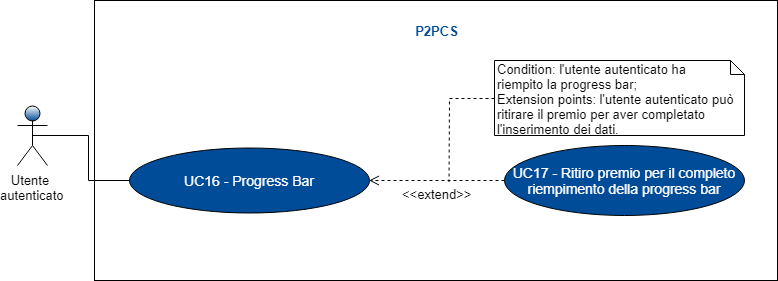
\includegraphics[width=13cm]{res/images/Schemagenerale7.png}
	\centering
	\caption{Schema generale: progress bar}
\end{figure}
\subsubsection{UC16 - Progress Bar}
\begin{itemize}
	\item \textbf{Attori Primari}: utente autenticato;
	\item \textbf{Descrizione}: l'utente che non ha ancora inserito tutti i suoi dati nel profilo visualizzerà una barra di avanzamento che si riempirà progressivamente in base ai dati inseriti;
	\item \textbf{Scenario principale}: l'utente apre la sezione \textit{Gestione Profilo} [UC14] e non ha ancora inserito tutti i dati possibili;
	\item \textbf{Estensioni}:
	\begin{itemize}
		\item ritiro del premio per il completo riempimento della progress bar [UC17].
	\end{itemize}
	\item \textbf{Precondizione}: l'utente autenticato non ha inserito tutti i dati possibili;
	\item \textbf{Postcondizione}: l'utente autenticato visualizza la progress bar.	
\end{itemize}

\subsubsection{UC17 - Ritiro premio per il completo riempimento della progress bar}
\begin{itemize}
	\item \textbf{Attori Primari}: utente autenticato;
	\item \textbf{Descrizione}: l'utente autenticato ha completato l'inserimento dei dati e può ritirare il relativo premio;	
	\item \textbf{Scenario principale}: l'utente autenticato ha riempito con successo la progress bar e gli compare la schermata per il ritiro della ricompensa;
	\item \textbf{Precondizione}: l'utente autenticato ha riempito la progress bar;
	\item \textbf{Postcondizione}: l'utente autenticato può ritirare il premio per aver completato l'inserimento dei dati.
\end{itemize}
